\documentclass[tikz,border=2pt]{standalone}
\usepackage{amsmath,amssymb}
\usepackage{pgfplots}
\pgfplotsset{compat=1.18}
\usetikzlibrary{calc}

\begin{document}
% Two independent dice: each has a flat pmf, but their sum is triangular, because the pmf of
% X + Y is the convolution P(X+Y=s) = sum_k P(X=k) P(Y=s-k).
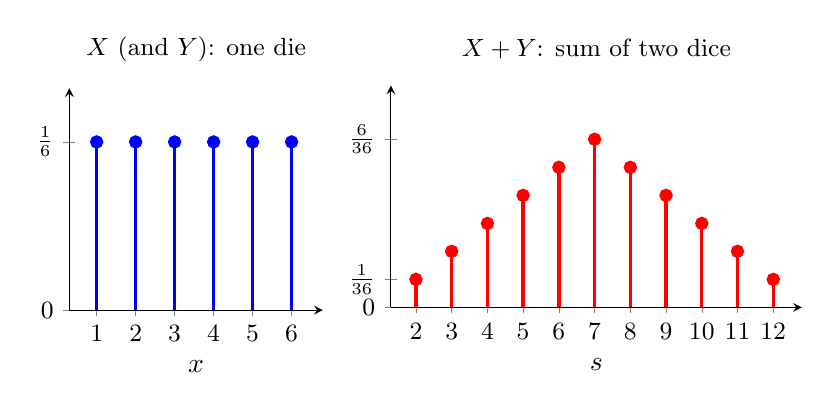
\begin{tikzpicture}
	\begin{axis}[name=p1, axis lines=left, xmin=0.3, xmax=6.8, ymin=0, ymax=0.22, xtick={1,...,6}, ytick={0,0.1667}, yticklabels={$0$,$\tfrac16$}, tick label style={font=\small}, xlabel={$x$}, width=4.8cm, height=4.4cm, clip=false, title={$X$ (and $Y$): one die}, title style={font=\small}]
		\addplot[ycomb, blue, very thick, mark=*, mark size=1.8pt] coordinates {(1,0.1667) (2,0.1667) (3,0.1667) (4,0.1667) (5,0.1667) (6,0.1667)};
	\end{axis}
	\begin{axis}[name=p2, at={(p1.outer east)}, anchor=outer west, xshift=2mm, axis lines=left, xmin=1.3, xmax=12.8, ymin=0, ymax=0.22, xtick={2,...,12}, ytick={0,0.0278,0.1667}, yticklabels={$0$,$\tfrac1{36}$,$\tfrac6{36}$}, tick label style={font=\small}, xlabel={$s$}, width=6.8cm, height=4.4cm, clip=false, title={$X+Y$: sum of two dice}, title style={font=\small}]
		\addplot[ycomb, red, very thick, mark=*, mark size=1.8pt] coordinates {(2,0.0278) (3,0.0556) (4,0.0833) (5,0.1111) (6,0.1389) (7,0.1667) (8,0.1389) (9,0.1111) (10,0.0833) (11,0.0556) (12,0.0278)};
	\end{axis}
	
\end{tikzpicture}
\end{document}
